\section{高速化に対する溶液濃度の影響}
\label{sec:concentration}
超音波照射による擬塑性流体中の落下球の高速化に対する溶液濃度の影響を調べる.実験条件をTable.\ref{table:exp-conditions}に示す.式(\ref{eq:Udiff})より,落下球高速化は球径の影響を受けることが示唆される.しかし,本実験条件では,球径の差が5\%程度にとどまることから,球径は同一として考える.

PAA溶液濃度と終端速度の関係をFig\ref{fig:concentrationUT}に示す.溶液濃度が高くなると,終端速度が遅くなる.超音波照射の有無による速度の比とPAA溶液濃度の関係を,Fig\ref{fig:concentrationUdiff}に示す.これらの結果より,縦軸を高速化度合,横軸を落下球の密度,溶液濃度の影響を考えた式(\ref{eq:UdiffRho})の右辺とした結果をFig\ref{fig:concentrationUdiff2}に示す.アルミニウム粒子では,濃度の上昇に伴い高速化度合が1.3程度となる正の相関が見られた.アルミナで粒子では,PAA濃度1.0wt.\%で高速化度合が1.2程度で最大となり,それ以上の濃度においては高速化度合が1に近づき,あまり高速化していない.ステンレス粒子では,濃度との相関が不明瞭であった.真鍮粒子では,PAA濃度0.7wt.\%の濃度で高速化度合が1.15程度で最大となった.これらをまとめた結果をFig\ref{fig:concentrationUdiffAll}に示す.超音波照射による速度比は,密度変化,粘度変化に対して弱い正の相関がみられた.高速化に対する溶液濃度の影響は存在するが,別の要因が生じているため弱い正の相関となったと考えられる.第\ref{sec:elasticity-discussion}章において,高速化への影響を与えていると考えられる,弾性による影響の議論を行う.

\begin{figure}[ht]
    \centering
    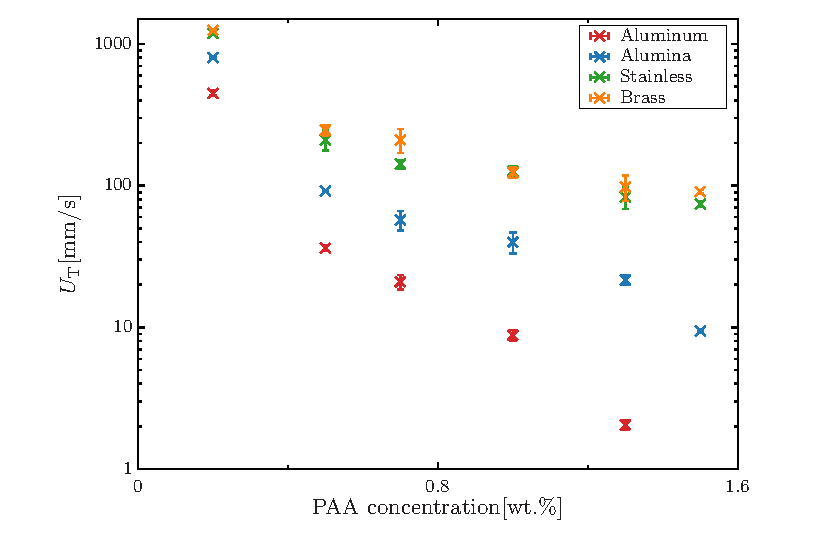
\includegraphics[width=0.8\textwidth]{./5-Results/concentrationUT.eps}
    \caption{Terminal velocity in PAA solution concentration.}
    \label{fig:concentrationUT}
\end{figure}

\begin{figure}[ht]
    \centering
    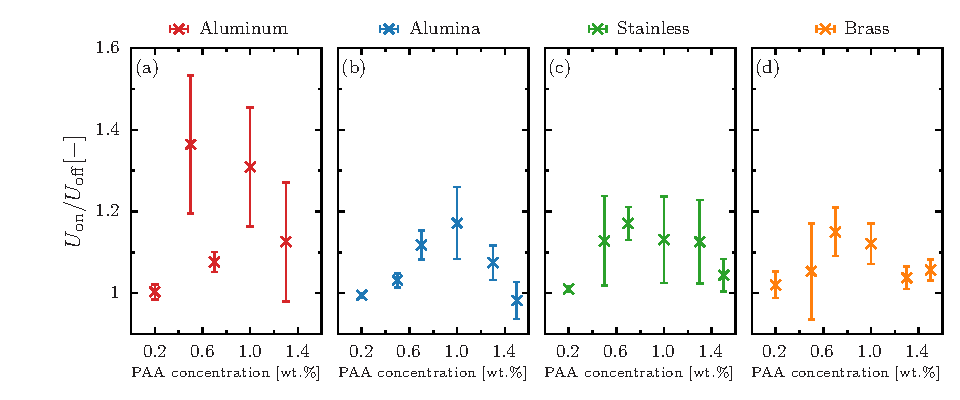
\includegraphics[width=1.0\textwidth]{./5-Results/concentrationUdiff.eps}
    \caption{Velocity ratio in PAA solution concentration (a)Aluminum, (b)Alumina, (c)Stainless, (d)Brass.}
    \label{fig:concentrationUdiff}
\end{figure}

\begin{figure}[ht]
    \centering
    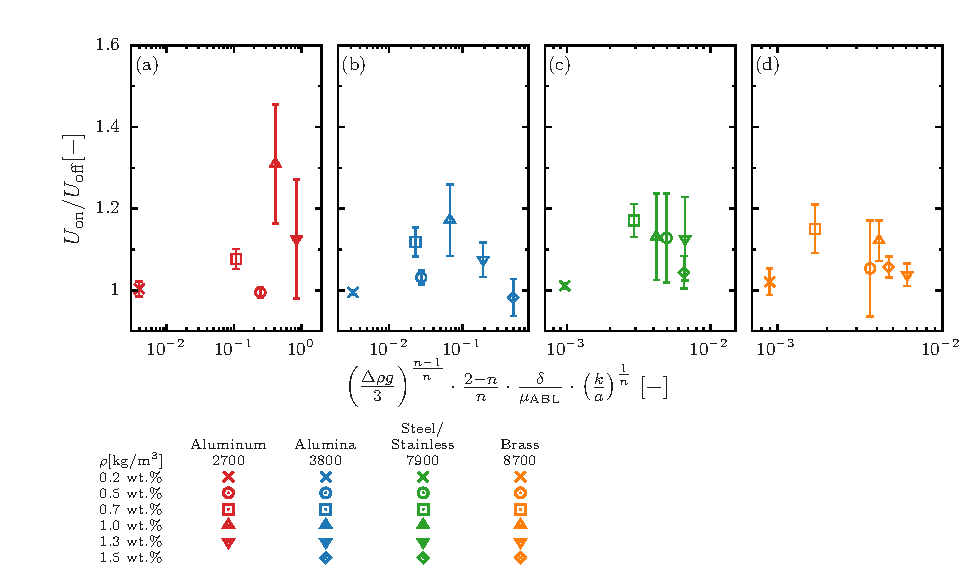
\includegraphics[width=1.0\textwidth]{./5-Results/concentrationUdiff_each.eps}
    \caption{Velocity ratio in PAA solution concentration (a)Aluminum, (b)Alumina, (c)Stainless, (d)Brass.}
    \label{fig:concentrationUdiff2}
\end{figure}

\begin{figure}[ht]
    \centering
    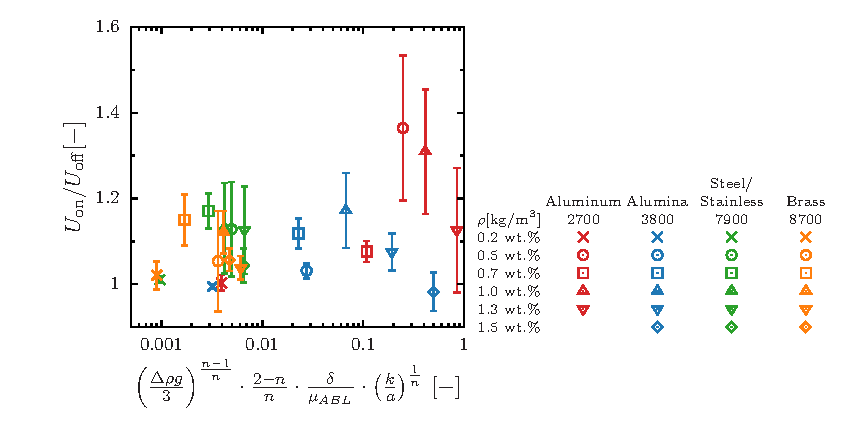
\includegraphics[width=0.7\textwidth]{./5-Results/concentrationUdiffAll.eps}
    \caption{Relationship between density, viscosity and terminal velocity.}
    \label{fig:concentrationUdiffAll}
\end{figure}